\documentclass[aspectratio=169,11pt]{beamer}

\usetheme[progressbar=frametitle, numbering=fraction]{metropolis}
\usepackage[T1]{fontenc}
\usepackage[utf8]{inputenc}
\usepackage[spanish,es-noshorthands,es-nodecimaldot,es-tabla]{babel}
\usepackage{amsmath,amssymb,mathtools}
\usepackage{booktabs}
\usepackage{tikz}
\usetikzlibrary{arrows.meta,positioning}
\graphicspath{{figuras/}}

\definecolor{rojo}{RGB}{214,39,40}
\definecolor{azul}{RGB}{33,102,194}
\definecolor{verde}{RGB}{102,190,102}
\definecolor{naranjo}{RGB}{255,127,14}
\setbeamercolor{alerted text}{fg=rojo}

\newcommand{\Z}{\mathbb{Z}}
\newcommand{\Lgen}{\mathcal{L}}
\DeclareMathOperator{\sgn}{sgn}
\newcommand{\ip}[2]{\langle #1,#2\rangle}
\newcommand{\norm}[1]{\lVert #1\rVert}
\newcommand{\repo}{https://github.com/martinmaturana777/Branching-Process-Complexes}
\newcommand{\video}[2]{\href{\repo/blob/main/videos/#1}{\small\textcolor{azul}{$\blacktriangleright$ #2}}}

\title{Procesos de ramificación en complejos celulares}
\subtitle{Simulación, extinción y conjuntos absorbentes}
\author{Martín Maturana Acevedo \and Bruno Guevara}
\institute{\footnotesize Simulación Estocástica · Universidad de Chile\\
Basado en el borrador \emph{Branching process on complexes} de D.~Cid y A.~Sepúlveda}
\date{Primavera 2026}

\begin{document}

\maketitle

\begin{frame}{Contenido}
  \tableofcontents
\end{frame}

%=====================================================================
\section{El problema}
%=====================================================================

\begin{frame}{De los grafos a los complejos}
  \begin{columns}[T]
    \begin{column}{0.55\textwidth}
      \begin{itemize}
        \item Un paseo aleatorio vive en los \textbf{vértices} de un grafo.
        \item Aquí las partículas viven en las \textbf{aristas} de $\Z^d$, y las que interactúan son las \textbf{caras} (cuadraditos).
        \item Cada arista $e$ tiene una carga entera $\theta_e\in\Z$:
        \begin{itemize}
          \item $\theta_e=3$: tres partículas \textcolor{rojo}{positivas};
          \item $\theta_e=-2$: dos partículas \textcolor{azul}{negativas}.
        \end{itemize}
        \item Configuración: $\theta\in\Z^{E}$, una 1-cadena entera.
      \end{itemize}
    \end{column}
    \begin{column}{0.42\textwidth}
      \centering
      \begin{tikzpicture}[scale=1.15]
        \foreach \x in {0,1,2,3} \draw[black!20] (\x,0) -- (\x,3);
        \foreach \y in {0,1,2,3} \draw[black!20] (0,\y) -- (3,\y);
        \draw[very thick, rojo] (1,1) -- (2,1); \fill[rojo] (1.5,1) circle (2pt);
        \draw[very thick, azul] (2,1) -- (2,2); \fill[azul] (2,1.5) circle (2pt);
        \draw[very thick, rojo] (0,2) -- (0,3); \fill[rojo] (0,2.5) circle (2pt);
        \fill[black!6] (1.05,1.05) rectangle (1.95,1.95);
        \node at (1.5,1.5) {\small $f$};
        \node[below] at (1.5,1) {\scriptsize $e$};
      \end{tikzpicture}
    \end{column}
  \end{columns}
\end{frame}

\begin{frame}{La dinámica: ramificación y aniquilación}
  \begin{columns}[c]
    \begin{column}{0.5\textwidth}
      \small
      Una partícula en $e$ hace \alert{sonar} una cara $f\ni e$:
      \[
        \theta\;\longmapsto\;\theta-\ip{e}{\partial f}\sgn(\theta_e)\,\partial f .
      \]
      \begin{itemize}
        \item La partícula se \textbf{aniquila} y nacen \textbf{3} en el resto del borde: \alert{ramificación} $1\to3$.
        \item Cargas opuestas en una arista se \textbf{cancelan}.
        \item Las que llegan al conjunto absorbente $T$ \textbf{mueren}.
      \end{itemize}
    \end{column}
    \begin{column}{0.47\textwidth}
      \centering
      \begin{tikzpicture}[scale=1.3]
        \fill[black!6] (0,0) rectangle (1,1);
        \draw[very thick, rojo] (0,0) -- (1,0); \fill[rojo] (0.5,0) circle (2pt);
        \draw[black!30] (1,0) -- (1,1) -- (0,1) -- (0,0);
        \node at (0.5,0.5) {$f$};
        \draw[-{Stealth}, thick] (1.25,0.5) -- (1.85,0.5);
        \begin{scope}[shift={(2.1,0)}]
          \fill[black!6] (0,0) rectangle (1,1);
          \draw[black!30] (0,0) -- (1,0);
          \draw[very thick, azul] (1,0) -- (1,1); \fill[azul] (1,0.5) circle (2pt);
          \draw[very thick, rojo] (0,1) -- (1,1); \fill[rojo] (0.5,1) circle (2pt);
          \draw[very thick, rojo] (0,0) -- (0,1); \fill[rojo] (0,0.5) circle (2pt);
          \node at (0.5,0.5) {$f$};
        \end{scope}
      \end{tikzpicture}
      \\[4mm]
      {\small una partícula $\Rightarrow$ tres partículas}
    \end{column}
  \end{columns}
\end{frame}

\begin{frame}{Lo que dice el paper}
  \begin{itemize}
    \item \textbf{Drift:} el generador cumple
      \[
        \Lgen I(\theta)=-\Delta_1^{\uparrow}\theta,\qquad \Delta_1^\uparrow=\partial_2\partial_2^T \ \text{(Laplaciano de Hodge superior)}.
      \]
      En promedio, la configuración se ``difunde y disipa''.
    \item \textbf{Lyapunov:} $\Lgen\norm{\theta}_2^2\le C_d\norm{\theta}_1-2\norm{\nabla\theta}_2^2$.
    \item \textbf{Extinción:} si se absorbe en un \alert{árbol generador} $T$, el proceso se extingue casi seguramente, con colas exponenciales.
  \end{itemize}
  \vspace{2mm}
  \begin{block}{Preguntas que quedan abiertas}
    ¿Cuánto tarda en extinguirse? ¿Qué pasa con menos aristas absorbentes, o con otras formas de $T$? ¿Y en 3D?
  \end{block}
\end{frame}

\begin{frame}{Nuestros objetivos}
  \begin{enumerate}
    \item Construir un \textbf{simulador exacto y eficiente} del proceso en $\Z^d$, para cualquier dimensión.
    \item \textbf{Verificar numéricamente} la teoría del paper (drift, Lyapunov, Poincaré).
    \item Estudiar la \alert{probabilidad de extinción}:
      \begin{itemize}
        \item ¿cuándo es posible?
        \item ¿cómo depende del \textbf{número de aristas absorbentes}?
        \item ¿cuánto tarda, en 2D y en 3D?
      \end{itemize}
    \item \textbf{Visualizar} la dinámica con videos en 2D y 3D.
  \end{enumerate}
\end{frame}

%=====================================================================
\section{El motor estocástico}
%=====================================================================

\begin{frame}{Representar el complejo con álgebra lineal}
  \begin{columns}[c]
    \begin{column}{0.58\textwidth}
      \begin{itemize}
        \item Cada celda se identifica con su \textbf{baricentro}. Al multiplicar por 2 queda en enteros: una $k$-celda tiene $k$ coordenadas impares.
        \item El borde $\partial_k$ es una \textbf{matriz rala}:
        \[
          \partial_kx=\sum_{i\in J_x}\varepsilon_{J_x}(i)\,(x^{+i}-x^{-i}).
        \]
        \item Chequeo clave: $\partial_1\partial_2=0$ exactamente, también en $\Z^3$.
        \item Absorción: $\partial_T=P_T\,\partial_2$, el borde sin las aristas de $T$.
      \end{itemize}
    \end{column}
    \begin{column}{0.38\textwidth}
      \centering
      \begin{tikzpicture}[scale=2, >=Stealth]
        \fill[black!6] (0,0) rectangle (1,1);
        \draw[->, very thick, rojo] (0,0) -- (1,0) node[midway, below] {\scriptsize $+$};
        \draw[->, very thick, rojo] (1,0) -- (1,1) node[midway, right] {\scriptsize $+$};
        \draw[->, very thick, azul] (0,1) -- (1,1) node[midway, above] {\scriptsize $-$};
        \draw[->, very thick, azul] (0,0) -- (0,1) node[midway, left] {\scriptsize $-$};
        \node at (0.5,0.5) {\small $\partial_2 f$};
      \end{tikzpicture}
      \\[2mm]{\scriptsize borde antihorario}
    \end{column}
  \end{columns}
\end{frame}

\begin{frame}{Simulación exacta: algoritmo de Gillespie}
  Cada par (partícula, cara vecina) tiene un reloj exponencial de tasa 1. La tasa total es $R=\sum_e|\theta_e|\,\lambda_e$.
  \vspace{2mm}
  \begin{enumerate}
    \item Esperar un tiempo $\tau\sim\mathrm{Exp}(R)$.
    \item Elegir la arista $e$ con probabilidad $|\theta_e|\lambda_e/R$ y luego una cara $f\ni e$ uniforme.
    \item Actualizar $\theta\leftarrow\theta-c\,\partial_Tf$. Solo cambian \textbf{4 aristas}, y la aniquilación es simplemente \textbf{suma en $\Z$}.
  \end{enumerate}
  \vspace{2mm}
  \begin{alertblock}{¿Por qué es exacto?}
    Si $X_i\sim\mathrm{Exp}(r_i)$ son independientes, entonces $\min_iX_i\sim\mathrm{Exp}(\sum_ir_i)$ y el reloj que suena primero es el $j$ con probabilidad $r_j/\sum_ir_i$. \textbf{No hay discretización del tiempo}: el único error es estadístico.
  \end{alertblock}
\end{frame}

\begin{frame}{Memoria, eficiencia y corridas largas}
  \begin{itemize}
    \item \textbf{Historial liviano:} se guarda solo qué cara sonó y con qué signo, que es el \emph{proceso de alturas} $\eta$. La trayectoria se reconstruye con una sola multiplicación matricial:
      \[
        \theta_t=\theta_0+\partial_T\,\eta_t .
      \]
    \item \textbf{Corridas de millones de eventos:} se guardan ``fotos'' del estado. Cuando se acumulan demasiadas, se descarta una de cada dos y se duplica el paso. La memoria queda acotada y las fotos equiespaciadas.
    \item \textbf{Paralelismo reproducible:} cada réplica tiene su propia semilla (\texttt{SeedSequence}), y el resultado es idéntico en serie y en paralelo.
    \item \textbf{Velocidad:} unos $10\,\mu$s por evento, es decir, $\sim10^8$ eventos en unos 15 minutos.
  \end{itemize}
\end{frame}

\begin{frame}{¿Cómo estimamos una probabilidad?}
  \begin{columns}[T]
    \begin{column}{0.6\textwidth}
      \small
      \textbf{Monte Carlo:} $R$ réplicas independientes; en cada una se observa si ocurre el evento, por ejemplo $\{\tau\le t^*\}$.
      \[
        \hat p=\frac{\#\{\text{réplicas en que ocurre}\}}{R}
      \]
      \[
        \text{error estándar}=\sqrt{p(1-p)/R}
      \]
      \begin{itemize}
        \item Cortar la simulación en $t^*$ \textbf{no sesga} el resultado: al cortar, ya se sabe si ocurrió el evento.
        \item Intervalos de \textbf{Wilson}, que funcionan bien aunque $\hat p$ sea 0 o 1.
      \end{itemize}
    \end{column}
    \begin{column}{0.36\textwidth}
      \small
      \begin{tabular}{@{}rr@{}}
        \toprule
        réplicas & IC 95\,\% \\
        \midrule
        300 & $\pm$5.7\,\% \\
        1000 & $\pm$3.1\,\% \\
        5000 & $\pm$1.4\,\% \\
        \bottomrule
      \end{tabular}\\
      {\scriptsize (peor caso, $p=\tfrac12$)}
      \vspace{3mm}

      \textbf{Verificaciones:}
      \begin{itemize}
        \item drift vs.\ $-\Delta^\uparrow\theta$: 0.55\,\% de error
        \item cota de Lyapunov en cada paso
        \item $\partial\partial=0$ exacto
      \end{itemize}
    \end{column}
  \end{columns}
\end{frame}

%=====================================================================
\section{Resultados}
%=====================================================================

\begin{frame}{La dinámica en 2D}
  \begin{columns}[c]
    \begin{column}{0.5\textwidth}
      \centering
      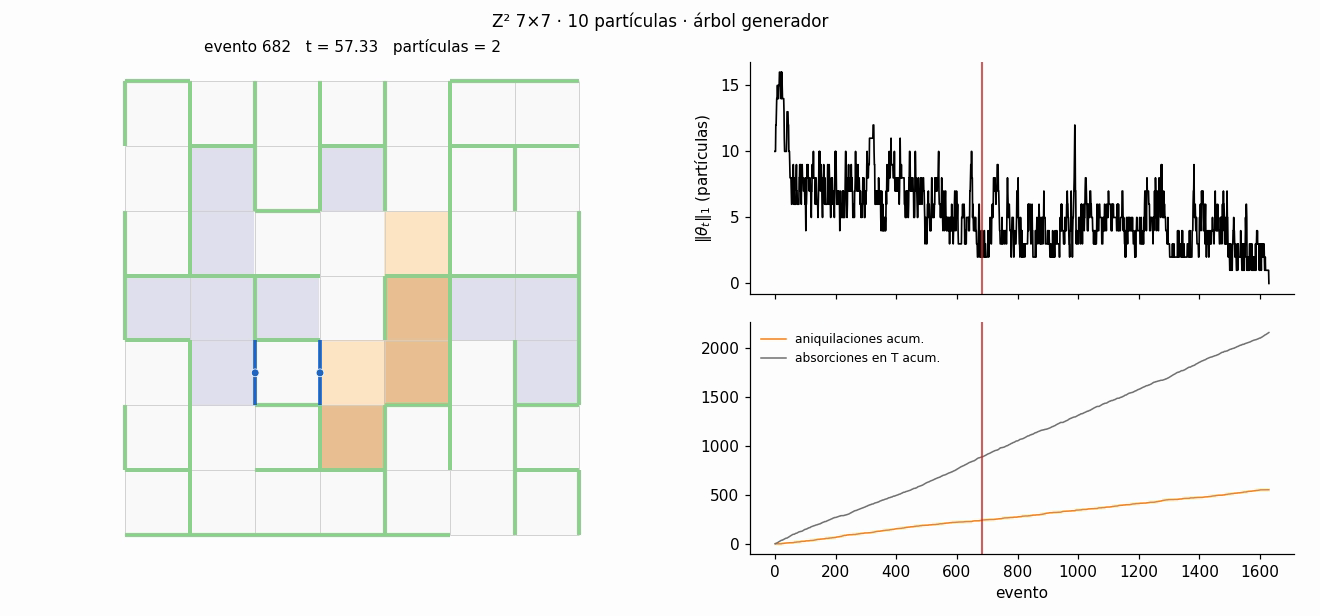
\includegraphics[width=\linewidth]{vid_z2_10particulas.png}\\
      {\scriptsize 10 partículas, absorción en un árbol (verde)}\\
      \video{z2_10particulas_arbol.mp4}{ver video}
    \end{column}
    \begin{column}{0.5\textwidth}
      \centering
      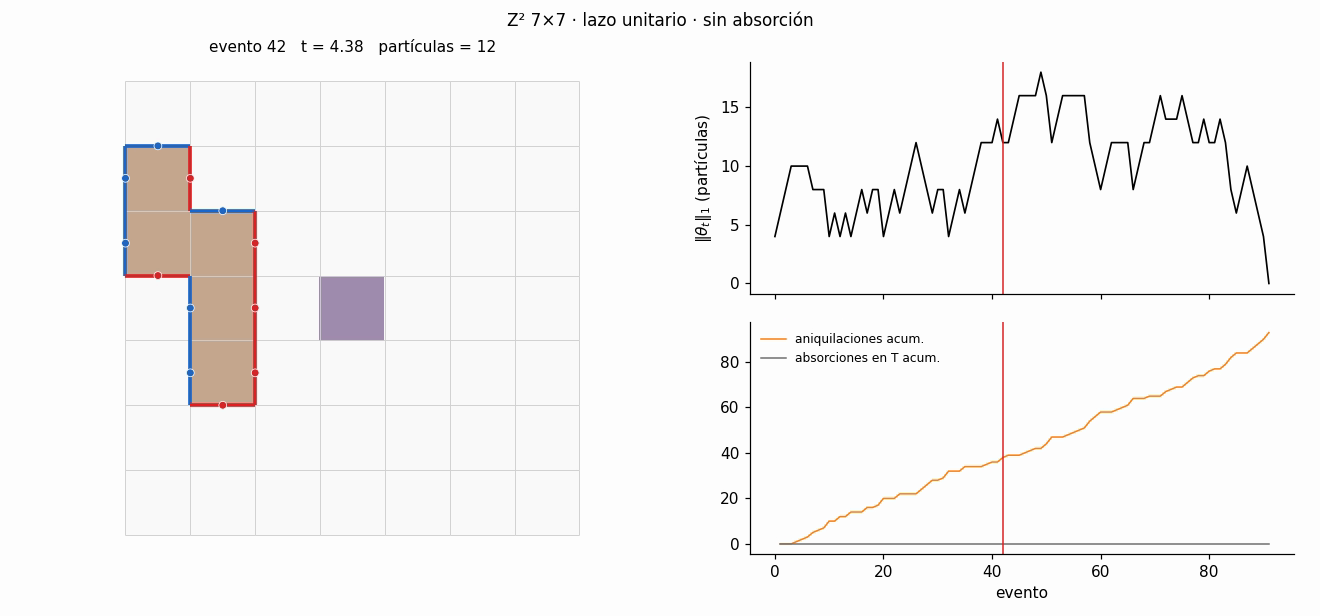
\includegraphics[width=\linewidth]{vid_z2_lazo_sin_arbol.png}\\
      {\scriptsize lazo sin absorción: las partículas son el \emph{borde} de una región}\\
      \video{z2_lazo_sin_arbol.mp4}{ver video}
    \end{column}
  \end{columns}
\end{frame}

\begin{frame}{Resultado principal: cargas conservadas}
  \begin{columns}[c]
    \begin{column}{0.47\textwidth}
      \small
      Para cada componente $C$ del grafo de aristas absorbentes, el flujo neto
      $Q_C=\sum_{v\in C}(\partial_1\theta)(v)$ \alert{se conserva}.
      \begin{itemize}
        \item Si algún $Q_C\neq0$, la extinción es \textbf{imposible}.
        \item Si todos son nulos, se extingue casi seguramente.
        \item Una partícula sobre $(u,w)$ se extingue $\iff$ $u$ y $w$ están \textbf{conectados} por $T$.
      \end{itemize}
    \end{column}
    \begin{column}{0.51\textwidth}
      \centering
      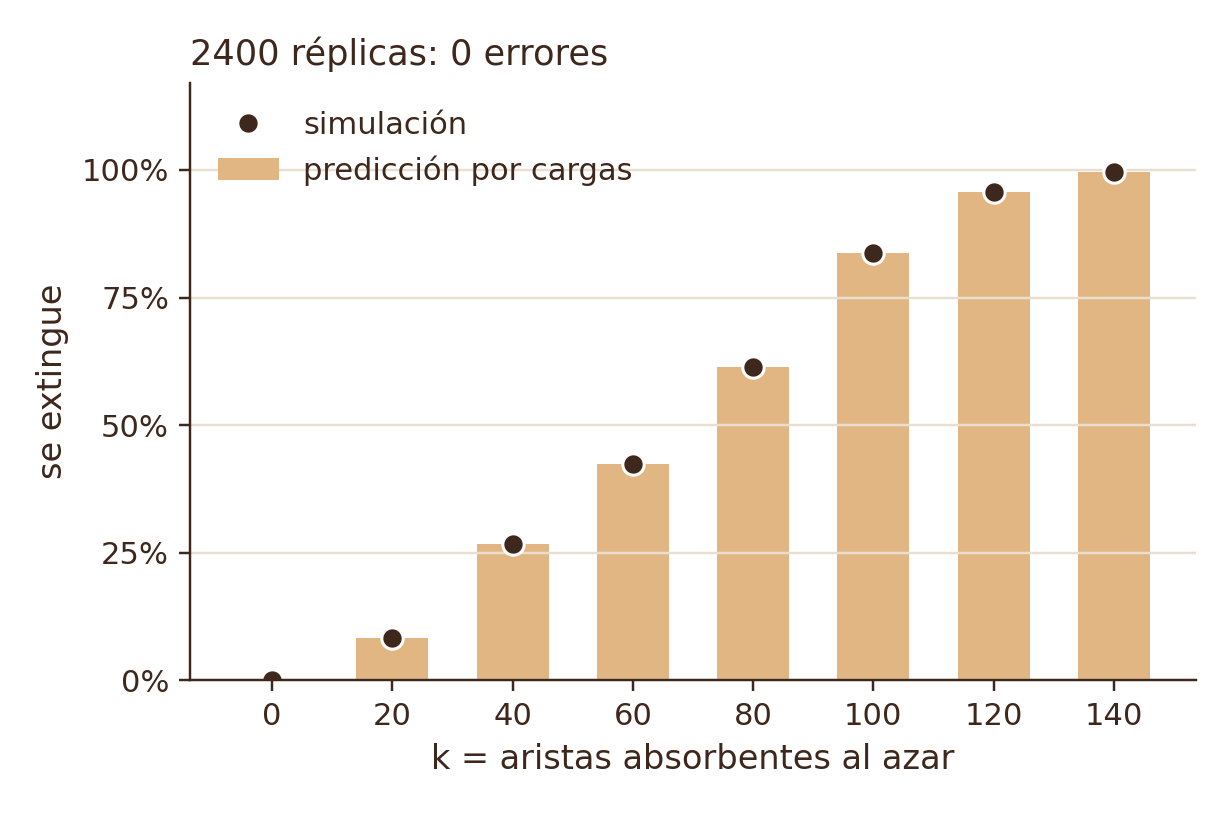
\includegraphics[width=\linewidth]{verificacion_cargas.png}\\
      {\scriptsize 2400 simulaciones: predicción $=$ observación, 0 errores}
    \end{column}
  \end{columns}
\end{frame}

\begin{frame}{Extinción eventual vs número de aristas absorbentes}
  \centering
  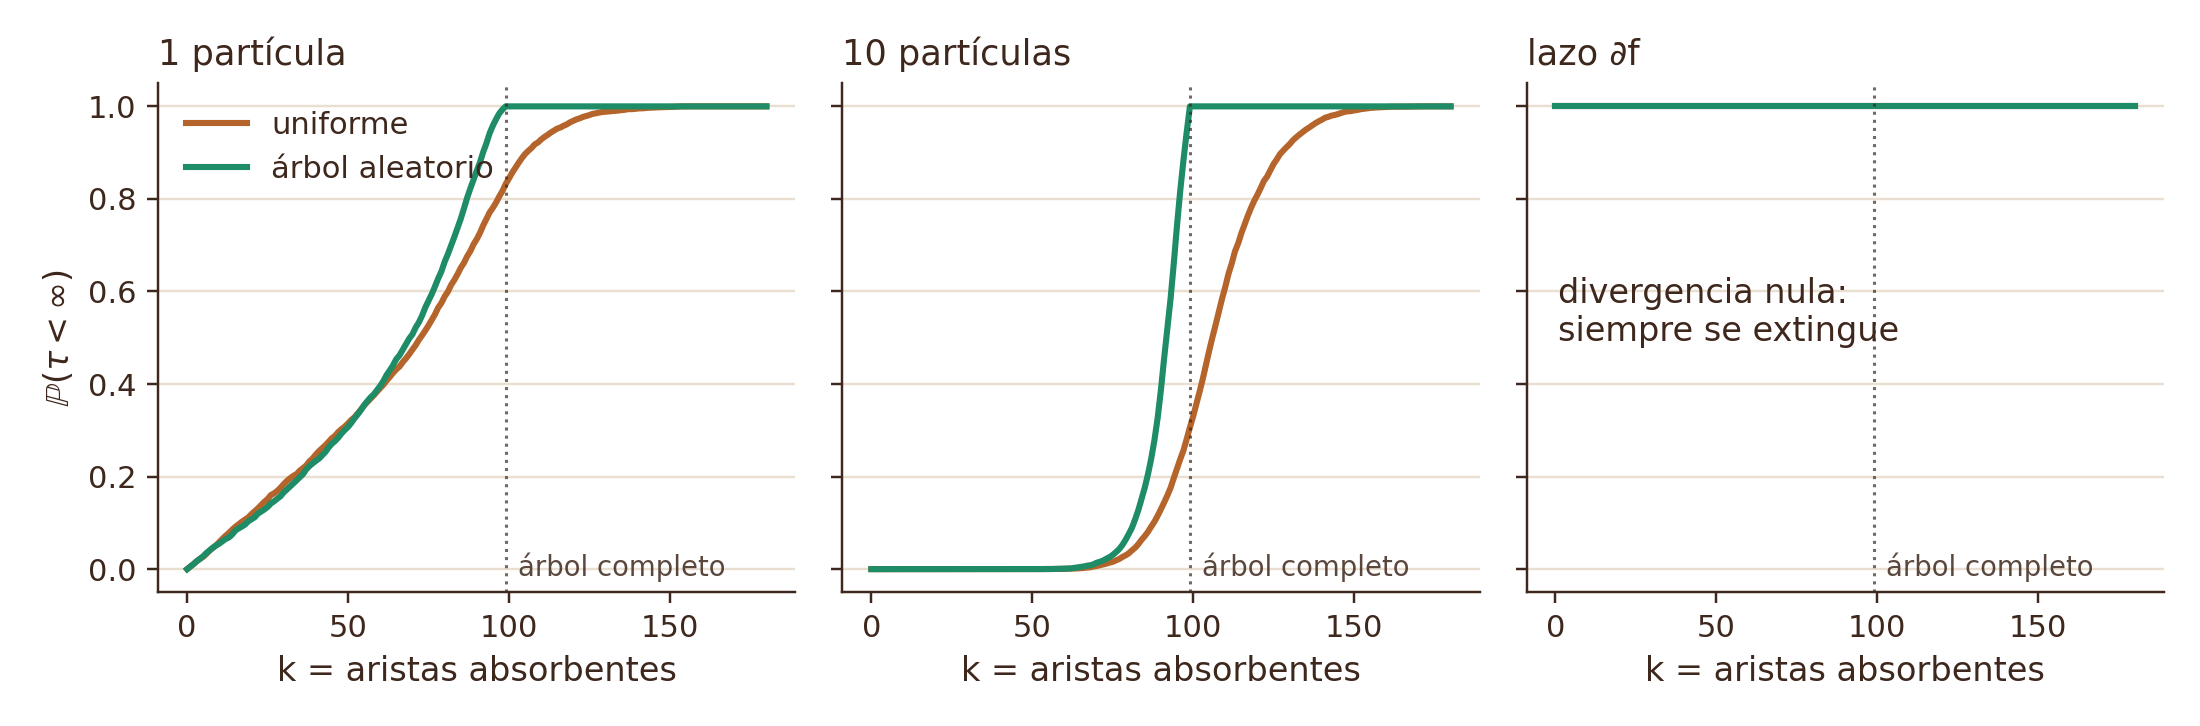
\includegraphics[width=0.98\textwidth]{aristas_exacta.png}
  \begin{itemize}\small
    \item Se calcula \textbf{exactamente} con las cargas, sin simular: es un problema de \emph{conectividad} (percolación).
    \item Es \textbf{monótona}: más aristas absorbentes, más probabilidad de extinción. El lazo se extingue siempre.
  \end{itemize}
\end{frame}

\begin{frame}{Sorpresa: en tiempo finito NO es monótona}
  \centering
  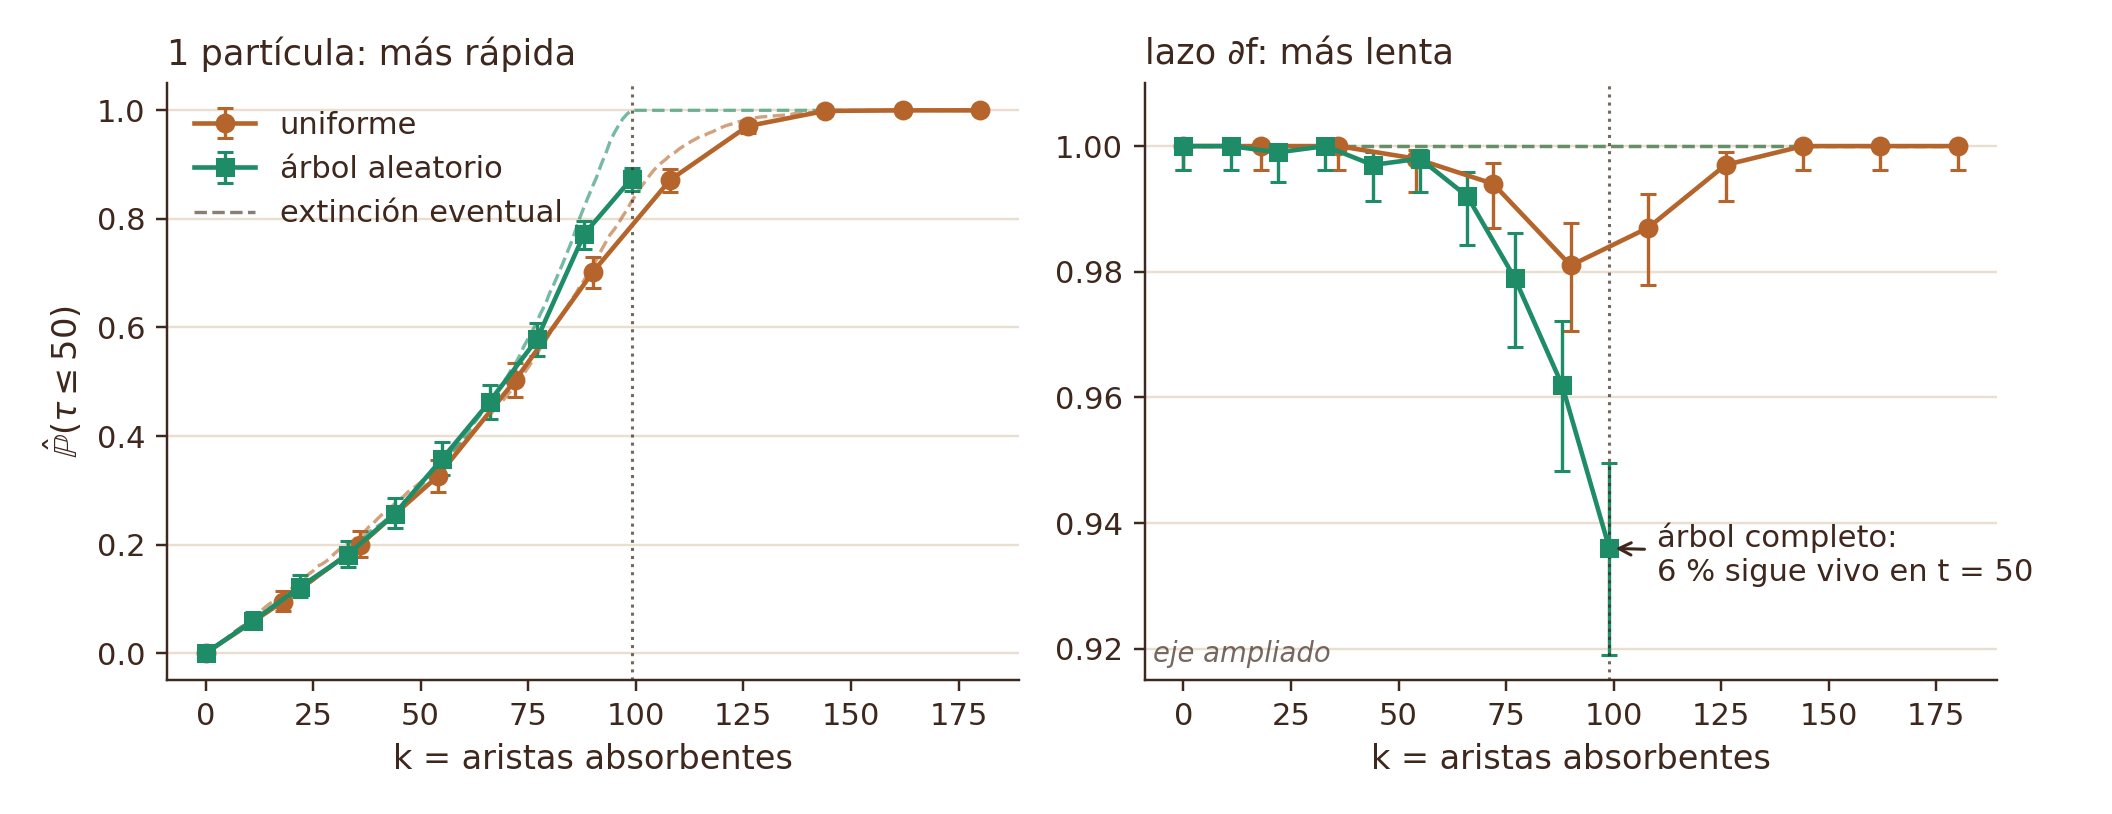
\includegraphics[width=0.85\textwidth]{aristas_tiempo_finito.png}
  \begin{itemize}\small
    \item Para el lazo, \alert{agregar aristas absorbentes hace más lenta la extinción}: $\mathbb{P}(\tau\le50)$ baja de 1.00 a 0.94.
    \item Hipótesis: absorber \emph{corta} el lazo en cadenas abiertas, cuyos extremos solo desaparecen al llegar a $T$.
  \end{itemize}
\end{frame}

\begin{frame}{Absorción que crece durante la simulación}
  \centering
  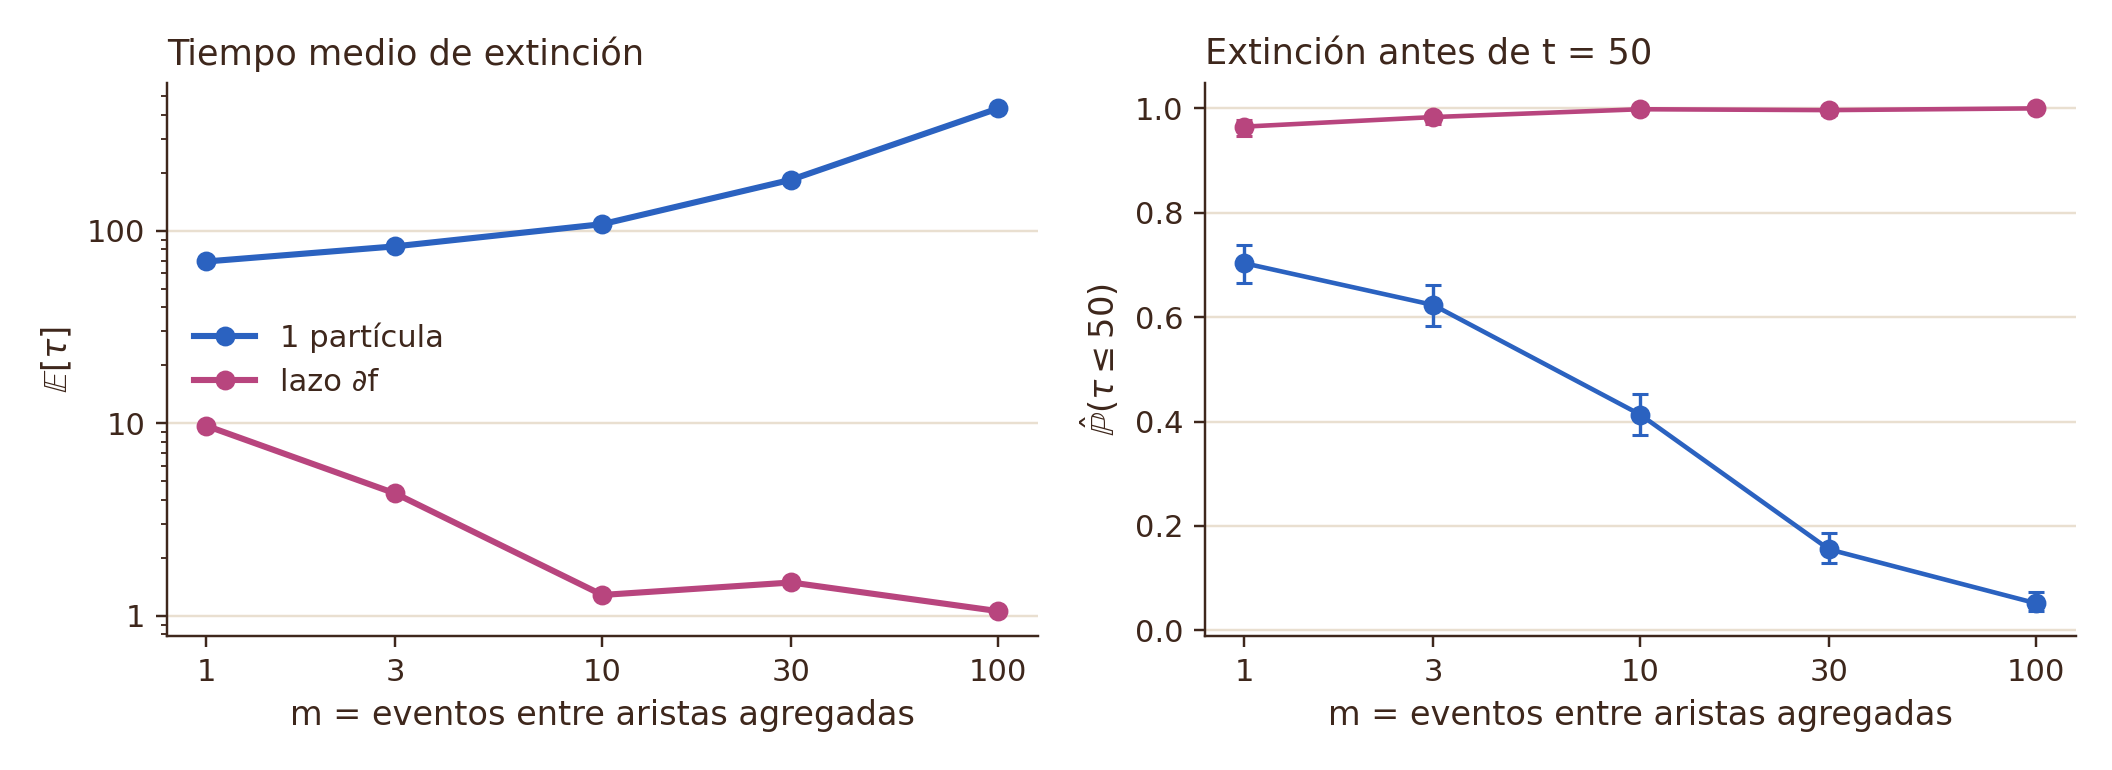
\includegraphics[width=0.85\textwidth]{aristas_dinamico.png}
  \begin{itemize}\small
    \item Se agrega una arista absorbente cada $m$ eventos.
    \item \textbf{Una partícula:} crecer rápido acelera la extinción ($\mathbb{E}[\tau]$: 69 con $m=1$, 432 con $m=100$).
    \item \textbf{Lazo:} lo contrario ($9.7$ frente a $1.1$). Si crece lento, el lazo alcanza a aniquilarse solo.
  \end{itemize}
\end{frame}

\begin{frame}{En 3D: la meseta}
  \begin{columns}[c]
    \begin{column}{0.5\textwidth}
      \centering
      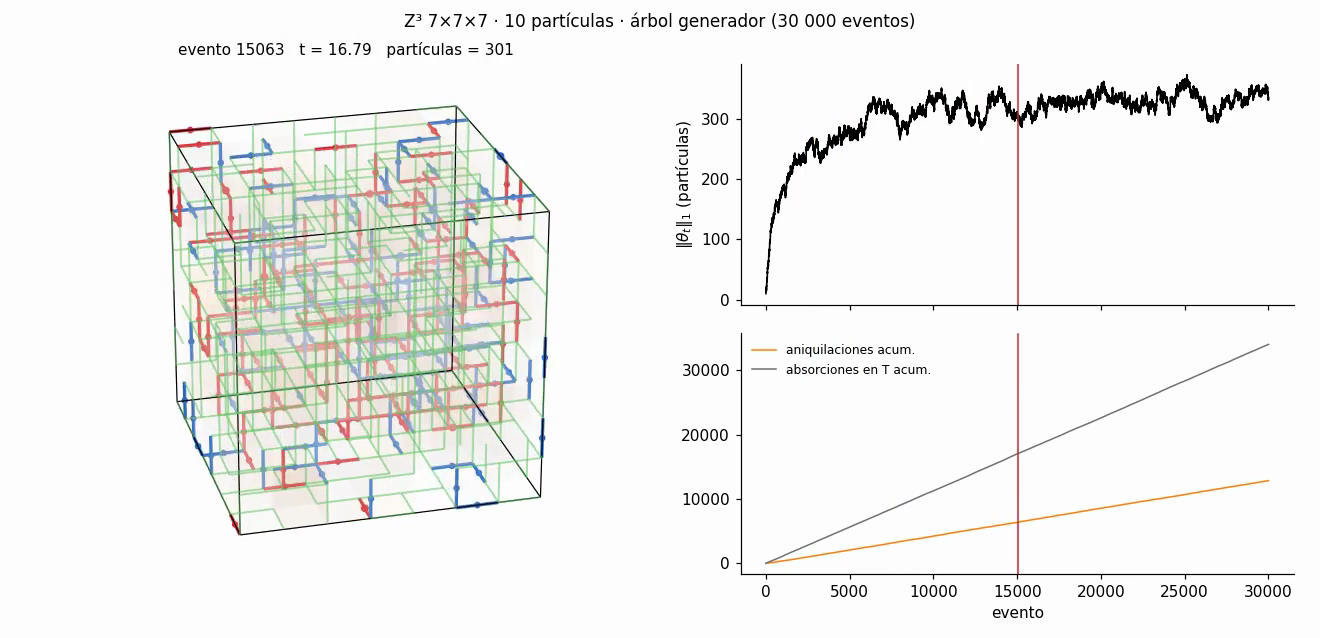
\includegraphics[width=\linewidth]{vid_z3_meseta.png}\\
      {\scriptsize $7\times7\times7$: crece a $\sim$370 partículas y se queda ahí}\\
      \video{z3_10particulas_arbol_meseta.mp4}{ver video}
    \end{column}
    \begin{column}{0.48\textwidth}
      \begin{itemize}
        \item En 3D la constante de Poincaré es diminuta, así que la deriva casi no empuja hacia abajo.
        \item El proceso queda en una \alert{meseta cuasi-estacionaria}.
        \item En $9^3$, la extinción \emph{temprana} (antes de 100 partículas) se satura en $\approx$0.3--0.4, aunque la extinción eventual sea segura.
      \end{itemize}
    \end{column}
  \end{columns}
\end{frame}

\begin{frame}{La corrida honesta: dejarla correr hasta que se extinga}
  \begin{columns}[c]
    \begin{column}{0.55\textwidth}
      \centering
      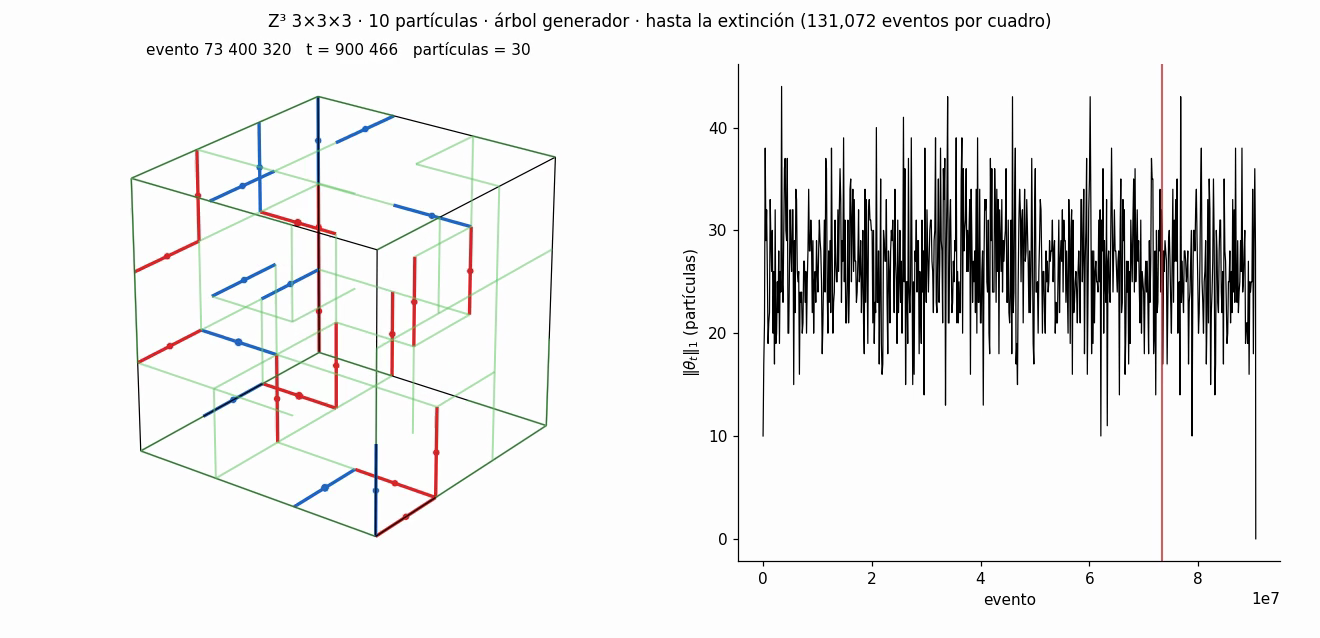
\includegraphics[width=\linewidth]{vid_z3_10particulas_extincion.png}\\
      \video{z3_10particulas_hasta_extincion.mp4}{ver video (cámara rápida)}
    \end{column}
    \begin{column}{0.43\textwidth}
      \small
      $3\times3\times3$, con árbol, \textbf{primera semilla, sin selección}:
      \vspace{1mm}

      \begin{tabular}{@{}lr@{}}
        \toprule
        corrida & eventos \\
        \midrule
        lazo & 23\,286\,239 \\
        10 partículas & \alert{90\,617\,992} \\
        \bottomrule
      \end{tabular}
      \vspace{2mm}

      \begin{itemize}
        \item Casi todo el tiempo en la meseta, y la caída final es \textbf{brusca}.
        \item Desde la meseta, el tiempo de extinción es $\approx$ \textbf{exponencial}: hay mucha variabilidad entre corridas.
      \end{itemize}
    \end{column}
  \end{columns}
\end{frame}

\begin{frame}{Una conjetura: la tasa de extinción es la constante de Poincaré}
  \centering
  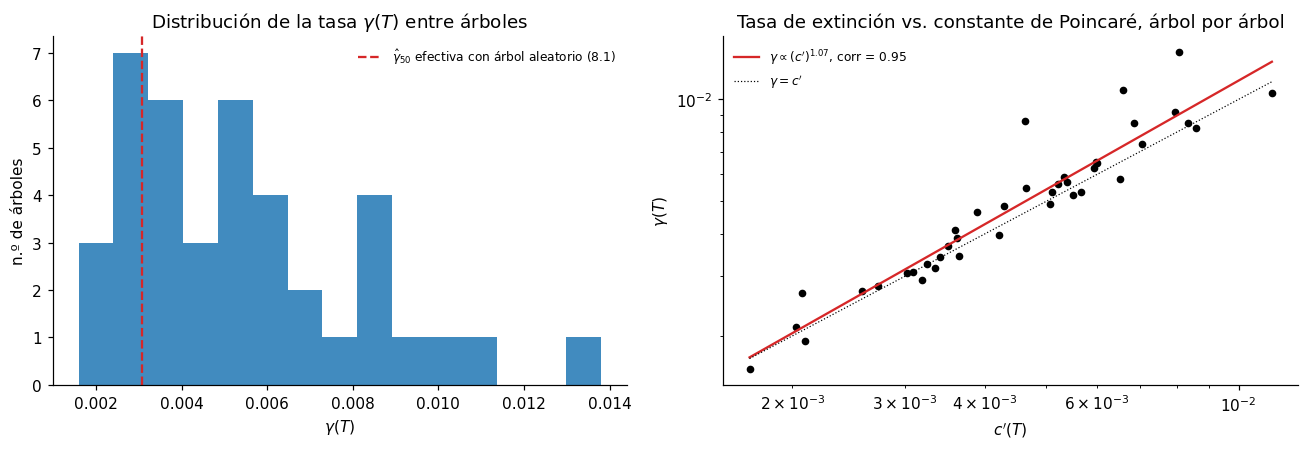
\includegraphics[width=0.85\textwidth]{ext_gamma_poincare.png}
  \begin{itemize}\small
    \item Con el árbol fijo, $\mathbb{P}(\tau>t)\approx Ce^{-\gamma(T)t}$, y la tasa $\gamma(T)$ \textbf{no depende} de la condición inicial.
    \item En 40 árboles: $\gamma(T)\approx c'(T)=\lambda_{\min}\big(\Delta^\uparrow|_{E\setminus T}\big)$, con correlación 0.95.
  \end{itemize}
\end{frame}

\begin{frame}{Conclusiones}
  \begin{enumerate}
    \item Construimos un simulador \textbf{exacto}, eficiente y reproducible en $\Z^d$, verificado contra la teoría.
    \item \alert{Cargas conservadas}: deciden si la extinción es posible y la convierten en un problema de conectividad.
    \item La extinción eventual es monótona en $T$, pero la \textbf{velocidad} de extinción no lo es.
    \item En 3D aparece una meseta cuasi-estacionaria: la extinción tarda decenas de millones de eventos incluso en $3\times3\times3$.
    \item Conjetura: la tasa de extinción coincide con la constante de Poincaré.
  \end{enumerate}
  \vspace{2mm}
  {\small Pendiente: demostrar la hipótesis de accesibilidad; usar el árbol uniforme (Wilson) y Fleming--Viot en 3D.}
\end{frame}

%=====================================================================
\section{Stochastic Ninja Warrior}
%=====================================================================

\begin{frame}{Stochastic Ninja Warrior}
  \centering
  {\large ¿Y si el conjunto absorbente \alert{se mueve}?}
  \vspace{1mm}

  \begin{columns}[T]
    \begin{column}{0.5\textwidth}
      \centering
      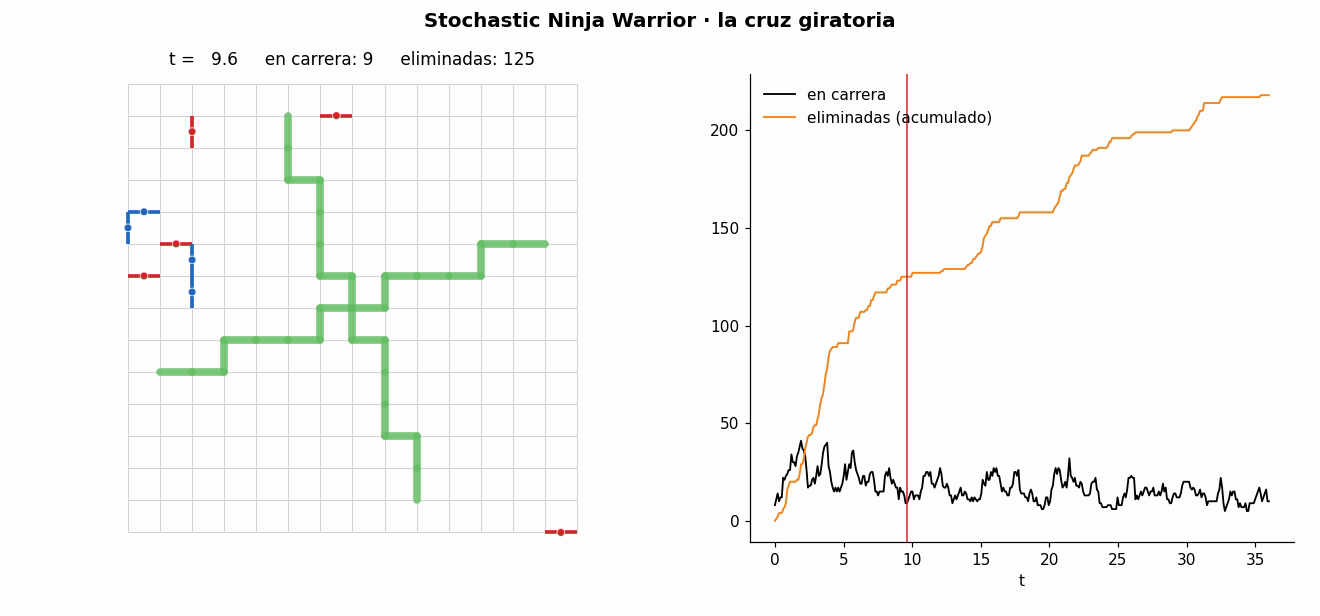
\includegraphics[width=\linewidth]{ninja_cruz.png}\\
      {\scriptsize la cruz giratoria}\\
      \video{ninja_cruz.mp4}{ver video}
    \end{column}
    \begin{column}{0.5\textwidth}
      \centering
      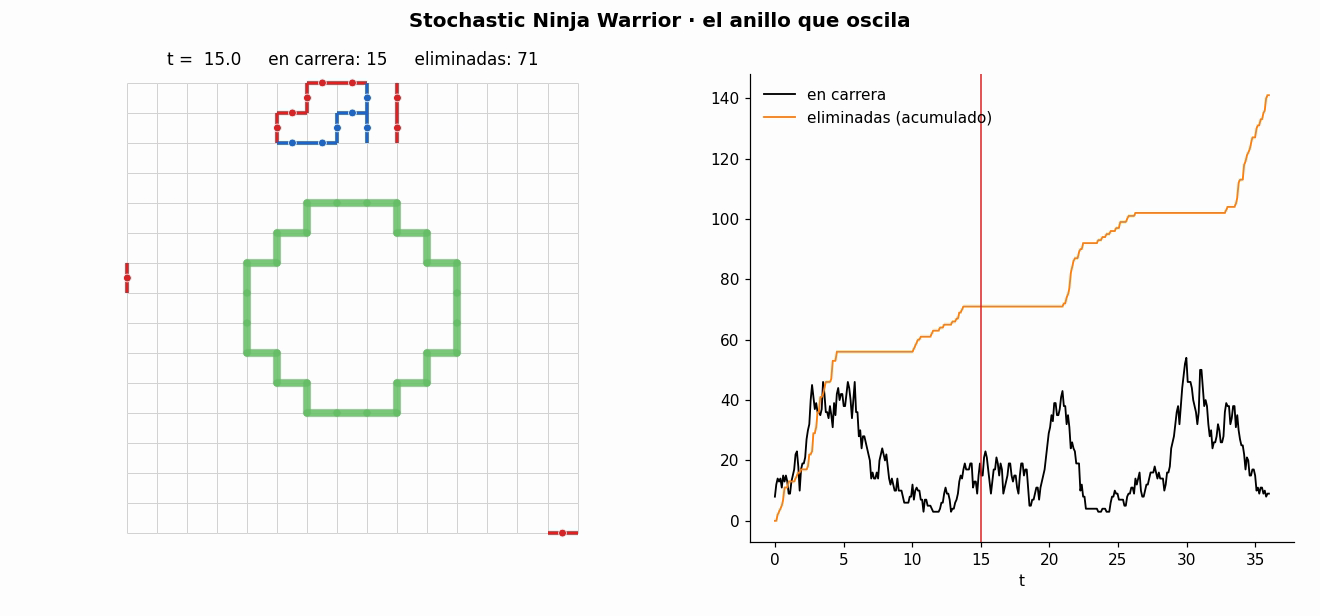
\includegraphics[width=\linewidth]{ninja_anillo.png}\\
      {\scriptsize el anillo que oscila hasta el lazo $\partial f$}\\
      \video{ninja_anillo.mp4}{ver video}
    \end{column}
  \end{columns}
  \vspace{2mm}
  {\small 8 concursantes $+1$; el obstáculo (verde) elimina a toda partícula que toca, y cada \textcolor{naranjo}{$\times$} marca una eliminación.}
\end{frame}

\begin{frame}{Stochastic Ninja Warrior: ¿quién sobrevive?}
  \begin{itemize}
    \item La simulación sigue siendo \textbf{exacta}: cada vez que el obstáculo se mueve, elimina lo que toca y el reloj se vuelve a sortear.
    \item Con un $T$ que se mueve, las cargas ya \textbf{no} se conservan, así que la extinción es posible.
    \item Aun así, nadie llega a GAME OVER: la ramificación y las eliminaciones se \textbf{equilibran}.
  \end{itemize}
  \vspace{2mm}
  \begin{center}
    \begin{tabular}{@{}lcc@{}}
      \toprule
      prueba (3 ciclos) & eliminadas & siguen en carrera \\
      \midrule
      cruz giratoria & 218 & 10 \\
      anillo que oscila & 141 & 9 \\
      \bottomrule
    \end{tabular}
  \end{center}
  {\small El anillo deja \emph{zonas seguras} en las esquinas.}
\end{frame}

\begin{frame}[standout]
  ¡Gracias!\\[4mm]
  {\normalsize ¿Preguntas?}\\[6mm]
  {\footnotesize \url{https://github.com/martinmaturana777/Branching-Process-Complexes}}
\end{frame}

\end{document}
